\documentclass[10pt]{article}
\usepackage{icmlko}

\icmlmeta{IP 파운데이션 월드모델}{182}{웹툰은 자기 과거를 못 쓴다}{노트 181이 ``풀링이 가정하는 라벨 동질성''을 남겼다. 전이 행렬을 그렸더니 판의 27\%인 도메인이 자기 역사로 자기 미래를 못 맞히고, 도서로 배우면 여덟 배 낫다}

\begin{document}

\twocolumn[
\icmlheader

\begin{abstract}
노트 181이 ``라벨이 다른 것을 묻는데 계수를 나눠 쓰나''를 제일 큰 줄로
남겼다. 재는 방법은 전이 행렬이다 --- 도메인 A 의 2025년 이전으로만
적합해 도메인 B 의 유보를 맞힌다. 여덟 도메인으로 그렸다. \textbf{대각선이
늘 이기지 않는다.} 다섯은 자기가 최고인데 \textbf{웹툰은 자기 전이가
$+$0.037 로 여덟 중 꼴찌}이고 도서로 배우면 $+$0.291, 웹툰으로 게임을
맞히면 $+$0.452 다. \textbf{판의 27\%를 차지하는 도메인이 자기 역사를 못
쓴다.} 왜인지 갈랐다. \textbf{\texttt{goods\_scale}(주당 회차 수)이 학습
$+$0.378에서 유보 $-$0.283 으로 부호를 뒤집는다} --- 덮음은 양쪽 다
100\%다. 능형은 2,106행에서 배운 큰 양의 계수를 들고 유보에 들어가 정확히
반대로 틀린다. \textbf{그런데 이건 유보를 안 봐도 보였다} --- 연도별로
2018년 $+$0.44 · 2021년 $+$0.58 · 2022년 $+$0.62 · 2023년 $+$0.51 ·
2024년 $+$0.36 으로 \emph{학습 구간 안에서} 이미 시들고 있다. 다만
\textbf{전체 기울기로는 못 잡는다}($-$0.002) --- 올랐다 내리므로 직선이
평평하다. \textbf{마지막 세 해 기울기로 잡는다}($-$0.129). 이걸 가드로
쓸 수 있나. 깃발로는 값이 있다 --- 걸린 축 열일곱의 유보 상관 변화 중앙이
$-$0.056 이고 나머지 마흔아홉은 $-$0.004 다. \textbf{그러나 규칙으로는 못
쓴다.} 문턱을 훑으니 F6 능형이 $-$0.05에서 $+$0.001, $-$0.10에서
\textbf{$+$0.024($t{=}2.9$)}, $-$0.15에서 \textbf{$-$0.030($t{=}-4.0$)},
$-$0.20에서 $+$0.000 이다 --- \textbf{한 칸 옆에서 부호가 뒤집히고 둘 다
갈린다.} 그리고 \textbf{끄기는 국소적이지 않다} --- 만화 · 세계애니의 축을
끄면 깃발에 없는 팝업이 $-$0.116 무너진다. \textbf{맨몸 가드는 통과한다}
(0.0\%). 가드 열둘이 못 잡는 실패 방식이다.
\end{abstract}
]

\begin{figure*}[t]
\centering
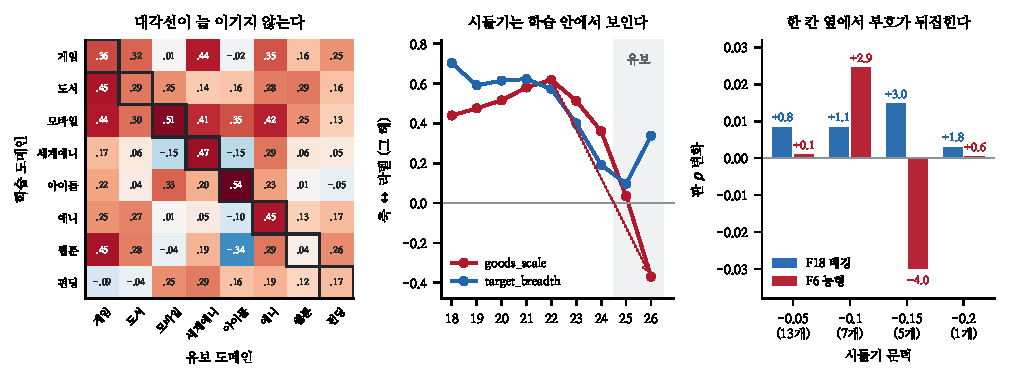
\includegraphics[width=\textwidth]{figs/past.pdf}
\caption{왼쪽 --- 대각선이 늘 이기지 않는다. 가운데 --- 시들기는 학습 안에서
보인다. 오른쪽 --- 한 칸 옆에서 부호가 뒤집힌다.}
\end{figure*}

\section{대각선이 늘 이기지 않는다}

\begin{table}[t]
\centering\tsize
\caption{공통 축 열아홉으로 능형. 행 도메인의 $<$2025 로 적합해 열 도메인의
$\ge$2025 를 맞힌다.}
\begin{tabular}{lrrl}
\toprule
유보 도메인 & 자기 & 최고 남 & \\
\midrule
\textbf{웹툰} & \textbf{$+$.037} & \textbf{$+$.291} & 도서 \\
게임 & $+$.364 & $+$.452 & 웹툰 \\
도서 & $+$.290 & $+$.319 & 게임 \\
펀딩 & $+$.171 & $+$.258 & 웹툰 \\
\midrule
모바일 & \textbf{$+$.506} & $+$.351 & 아이돌 \\
아이돌 & \textbf{$+$.545} & $+$.351 & 모바일 \\
세계애니 & \textbf{$+$.470} & $+$.436 & 게임 \\
애니 & \textbf{$+$.450} & $+$.421 & 모바일 \\
\bottomrule
\end{tabular}
\end{table}

\claimx{\textbf{웹툰은 전부에게 진다.} 자기 전이 $+$0.037 인데 여섯 도메인이
그보다 낫게 맞힌다. 학습 2,106행 · 유보 711행으로 표본 문제가
아니다.}{\textbf{그러니 풀링이 웹툰을 살리고 있다} --- 노트 181이 ``라벨이
다른데 계수를 나눠 쓰나''를 걱정했는데, 적어도 한 도메인에서는 나눠 쓰는
것이 유일한 구제책이다.}

\claimx{\textbf{전이가 대칭이 아니다.} 웹툰$\to$게임이 $+$0.452 인데
게임$\to$웹툰은 $+$0.160 이다. 웹툰의 \emph{과거}는 남을 가르치는 데 쓸 수
있고 자기 \emph{미래}에는 못 쓴다.}{그러면 웹툰의 문제는 축이 나쁜 것이
아니라 \textbf{시점이 옮겨간 것}이다.}

\section{한 축이 부호를 뒤집는다}

\begin{table}[t]
\centering\tsize
\caption{웹툰 축 $\leftrightarrow$ 라벨. 덮음은 양쪽 다 100\%.}
\begin{tabular}{lrrr}
\toprule
& 학습 & 유보 & 차 \\
\midrule
\textbf{goods\_scale} & \textbf{$+$.378} & \textbf{$-$.283} & \textbf{$-$.661} \\
cal\_holiday\_gap & $+$.127 & $-$.071 & $-$.198 \\
entry\_friction & $+$.129 & $+$.301 & $+$.172 \\
target\_breadth & $+$.319 & $+$.235 & $-$.083 \\
\bottomrule
\end{tabular}
\end{table}

\claimx{\textbf{덮음이 안 변하는데 부호가 뒤집힌다.} 노트 174가 다룬
비대칭(덮음이 시간에 무너짐)과 다른 종류다 --- 여기서는 열이 멀쩡히
있는데 \emph{뜻이} 바뀐다.}{\texttt{goods\_scale} 은 웹툰에서 주당 회차
수다(\texttt{docs/AXIS\_MEANING.md}). 2018$\sim$2022년에는 많이 올리는
작품이 즐겨찾기를 많이 받았고 2026년에는 반대다. \textbf{플랫폼이
바뀌었다.}}

\section{유보를 안 보고도 보였다}

\begin{table}[t]
\centering\tsize
\caption{웹툰 \texttt{goods\_scale} 의 연도별 상관.}
\begin{tabular}{lrrrrrr}
\toprule
& '20 & '21 & \textbf{'22} & '23 & '24 & \\
\midrule
학습 & .52 & .58 & \textbf{.62} & .51 & .36 & \\
\midrule
& \multicolumn{2}{c}{'25} & \multicolumn{2}{c}{'26} & & 유보 \\
& \multicolumn{2}{c}{.04} & \multicolumn{2}{c}{\textbf{$-$.37}} & & \\
\bottomrule
\end{tabular}
\end{table}

\claimx{\textbf{2022년에 봉우리를 치고 학습 구간 안에서 이미 내려온다.}
2023년 $+$0.51 · 2024년 $+$0.36 --- 유보를 한 칸도 안 보고 잴 수 있는
값이다.}{그래서 ``시점''을 새로 쓸 수 있다 --- 노트 141의 시점 층은
``자질이 오픈 이전에 존재했나''를 봤고, 여기서는 \textbf{``자질과 라벨의
관계가 아직 살아 있나''}를 본다.}

\claimx{\textbf{전체 기울기로는 못 잡는다}($-$0.002). 2018$\sim$2022년에
오르고 2023$\sim$2024년에 내리므로 직선이 평평하다. \textbf{마지막 세 해
기울기가 잡는다}($-$0.129) --- 예순여섯 개 중 둘째로 가파르다.}{\textbf{내
첫 통계가 틀렸다.} 처음에 전체 기울기로 재고 ``상관 $+$0.288''을 얻었는데,
정작 제일 크게 무너진 축이 목록에 없었다. \textbf{노트 133의 규칙이 내
통계에도 걸린 것이다.}}

\section{깃발로는 되고 규칙으로는 안 된다}

\begin{table}[t]
\centering\tsize
\caption{학습 구간에서 시드는 축의 유보 상관 변화.}
\begin{tabular}{lrr}
\toprule
& 개수 & 변화 중앙 \\
\midrule
\textbf{시듦} (최근 기울기 $<-$.03) & 17 & \textbf{$-$.056} \\
나머지 & 49 & $-$.004 \\
\bottomrule
\end{tabular}
\end{table}

\begin{table}[t]
\centering\tsize
\caption{그 축들을 끄면. 문턱을 훑는다.}
\begin{tabular}{lrrr}
\toprule
문턱 & 끈 수 & F18 배깅 & F6 능형 \\
\midrule
$-$0.05 & 13 & $+$.0084 & $+$.0010 \\
\textbf{$-$0.10} & 7 & $+$.0084 & \textbf{$+$.0244} \\
\textbf{$-$0.15} & 5 & $+$.0148 & \textbf{$-$.0299} \\
$-$0.20 & 1 & $+$.0030 & $+$.0004 \\
\bottomrule
\end{tabular}
\end{table}

\claimx{\textbf{한 칸 옆에서 부호가 뒤집히고 둘 다 갈린다} --- $-$0.10 에서
$+$0.0244($t{=}2.9$)이고 $-$0.15 에서 $-$0.0299($t{=}-4.0$)다. 그 사이에
축 둘이 더 빠질 뿐이다.}{\textbf{그러니 이 이득은 못 채택한다.} 웹툰 두
축만 끄면 F6 이 $+$0.0238($t{=}3.1$)로 이 흐름 최대인데, \textbf{``웹툰만''을
고른 것 자체가 판을 보고 고른 것이다.}}

\section{그리고 국소적이지 않다}

\begin{table}[t]
\centering\tsize
\caption{무엇을 끄느냐에 따른 도메인 $\rho$(F18).}
\begin{tabular}{lrrr}
\toprule
& 팝업 & 게임 & 세계애니 \\
\midrule
현행 & .343 & .468 & .549 \\
웹툰 둘만 & .323 & .458 & .558 \\
\textbf{만화·세계애니} & \textbf{.226} & \textbf{.593} & .457 \\
전부 & \textbf{.127} & .587 & .454 \\
\bottomrule
\end{tabular}
\end{table}

\claimx{\textbf{팝업은 깃발에 한 번도 안 걸리는데 $-$0.116 · $-$0.215
무너진다.} 만화 · 세계애니가 손 축 셋씩 잃으면 풀링 계수가 얇아지고, 유보
59건뿐인 팝업이 그 계수에 제일 크게 기댄다.}{반대로 게임은 $+$0.125
오른다. \textbf{순이득이 아니라 재배분이다} --- 판 전체는 $+$0.0084 인데
그 안에서 도메인 하나가 반 토막 난다.}

\claimx{\textbf{맨몸 가드는 통과한다}(0.0\%). 노트 174가 세운 규약은 ``유보
레코드에 손 축이 0개면 안 된다''인데 팝업은 다섯을 다 갖고 있다 ---
\textbf{자기 축이 멀쩡해도 남의 축이 빠지면 무너진다.} 가드 열둘이 못
잡는 실패 방식이다.}{노트 174가 ``빠진 축이 아니라 남은 축을 봐야
했다''고 적었는데, 이번에는 \textbf{남의 남은 축}까지 봐야 한다.}

\begin{table}[t]
\centering\tsize
\caption{남은 것.}
\begin{tabular}{ll}
\toprule
\textbf{가드} & 남의 축을 끌 때 내 도메인이 무너지는 것 \\
웹툰 & 시점 이동을 자질로 다룰 것인가 \\
전이 & 대칭이 아닌 까닭 --- 표본 크기인가 시점인가 \\
\bottomrule
\end{tabular}
\end{table}

첫 줄이 곧바로 만들 수 있다. 축을 끄거나 켤 때마다 \emph{모든} 도메인의
$\rho$ 를 재고 어느 하나가 문턱 넘게 내려가면 막는 가드다 --- 이번 실험에서
팝업이 0.343에서 0.127로 갔는데 판은 오히려 올랐고, 판만 보면 통과했을
것이다. \textbf{판은 크기 가중 평균이라 작은 도메인이 무너지는 것을 숨긴다.}

\end{document}
